\chapter[Methodology]{Methodology}
\label{Chap:Methodology}

% ***************************************************
% Methodology
% ***************************************************

% ********* Enter your text below this line: ********

\section{SC-LIO-SAM Pipeline}
SC-LIO-SAM extends the LIO-SAM LiDAR–inertial estimator by injecting Scan Context loop closure constraints while retaining the tightly coupled factor-graph back end described by Shan et al. \cite{shan_2020_liosam}. Incoming MulRan scans \cite{kim_2020_mulran} are first deskewed using high-rate IMU measurements, projected into a range image, and segmented into planar and edge features. The mapping module maintains two voxel grids: one for surf feature downsampling and another for corner features. Both grids feed the scan-to-map optimisation and the ICP residual update, so their leaf sizes directly control how many constraints participate in every Gauss–Newton iteration. Loop closures generated via Scan Context \cite{gkim-2018-iros} enter the graph as pose constraints that limit long-term drift without breaking real-time guarantees.

The \texttt{mapping\_surf\_leaf\_size} parameter governs the size of the voxel filter used for surf points inside \texttt{mapOptimization}. Smaller values densify the surf map and reduce alignment error at the cost of higher computation per frame, whereas larger values encourage faster execution with lower fidelity. Because the parameter is exposed as a ROS topic, SC-LIO-SAM can accept new values at runtime without recompilation, making it a viable actuator for a reinforcement learning (RL) controller.

\section{ROS Replay and Integration}
Training and evaluation happen inside reproducible ROS sessions that continuously replay MulRan sequences via the headless file player. The \texttt{EpisodeOrchestrator} module coordinates a persistent ROS core—hosting rosbridge and the metrics exporter—and per-episode launches for SC-LIO-SAM, the MulRan player, and the TUM logger. Each reset randomises the selected sequence (KAIST01 or Riverside01) and the playback start percentage, publishes a safe surf leaf size, and waits for the metrics exporter to confirm that valid statistics are available before unpausing the RL loop.

The metrics exporter subscribes to \texttt{/lio\_sam/deskew/cloud\_deskewed}, \texttt{/feature/cloud\_{surface,corner}}, \texttt{/imu/data\_raw}, and \texttt{/lio\_sam/mapping/odometry\_incremental}. It maintains running statistics, variable-length scan tokens, and a critique tail, writing everything to \path{/tmp/rlvo/metrics.json} whenever the RL process calls \texttt{/rl\_metrics/commit} through rosbridge. Concurrently, \texttt{odom\_to\_tum.py} records the incremental odometry topic into \texttt{est.tum} files so that absolute pose error (APE) can be computed.

\begin{figure}[H]
\centering
\includegraphics[width=\textwidth]{Chapter3/ros_data_flow.png} 
\caption{ROS-native replay stack linking MulRan data, SC-LIO-SAM, and the RL environment.}
\label{fig:ros_data_flow}
\end{figure}


\section{Reinforcement Learning Environment}
The RL host runs outside ROS and observes only the artefacts exported by the replay stack. Its logic resides in \texttt{rl\_vo/env/rl\_env.py} and is responsible for translating ROS metrics into observations, mapping PPO actions into voxel sizes, and computing data-driven rewards.

\subsection{Observation Design}
Each step aggregates three components produced by the metrics exporter:
\begin{itemize}
  \item \textbf{Fixed scalars} covering scan statistics, surf and corner feature counts, odometry cadence, inertial root-mean-square values, planarity proxies, and the previous action. These signals summarise estimator health and motion context.
  \item \textbf{Variable tokens} built from sequences of $(\texttt{surf\_pts}, \texttt{corner\_pts}, \texttt{vel\_norm})$ tuples. Up to 64 tokens capture short-term dynamics so the attention backbone can reason over trends rather than isolated scalars.
  \item \textbf{Critique tail} consisting of four extra values appended to the critic input only, providing additional context about scan rates and dropouts that stabilise value estimation.
\end{itemize}

\texttt{RunningMeanStdLite} maintains an online normaliser for all observation dimensions. Normalisation updates occur only when the metrics exporter confirms that a commit succeeded, preventing NaNs during ROS start-up transients. The validation environment regularly copies these statistics so evaluation rollouts use the same scaling as training.

\subsection{Action Channel and Safety}
The policy outputs a single scalar $a_t \in [0,1]$. The helper \texttt{action\_to\_leaf()} logarithmically interpolates this value into the physical range $[5\times10^{-4},\,1.0]$~m, ensuring that uniform policy outputs correspond to meaningful changes in voxel resolution. \texttt{EpisodeOrchestrator} publishes the result to \texttt{/lio\_sam/params/mapping\_surf\_leaf\_size} via rosbridge, and the metrics exporter mirrors the latest action in the observation vector so PPO can penalise sharp jumps. During resets, the orchestrator enforces a default value of $0.40$~m until valid observations become available, guarding against destabilising SC-LIO-SAM while ROS processes initialise.

\subsection{Reward Shaping}
Rewards combine pose accuracy, runtime penalties, and action smoothness:
\begin{equation}
  r_t = -0.1 \cdot \text{APE}_t - 0.001 \cdot \Delta t_t - 0.01 \cdot \lvert a_t - a_{t-1} \rvert,
\end{equation}
where $\text{APE}_t$ is the root-mean-square positional error computed by the evo toolkit over the last three seconds of TUM logs \cite{grupp2017evo}, and $\Delta t_t$ captures the latency observed by the orchestrator during the most recent step. This structure rewards lower trajectory error, discourages overly small voxels that would stall SC-LIO-SAM, and promotes smooth parameter schedules reminiscent of the PPO tuning approach used for visual odometry \cite{nicomessikommer_2024_reinforcement}. When MulRan ground truth or ROS metrics are unavailable, the environment emits a zero reward together with an invalid mask so the PPO buffer discards the transition.

\section{Hyperparameter Sweep Methodology}
Before integrating RL, the pipeline executed one-factor-at-a-time sweeps across the dominant SC-LIO-SAM parameters. The sweep script cloned the canonical MulRan configuration, substituted candidate values using \texttt{yq}, and launched \texttt{run\_eval\_ros1.sh} to replay KAIST01 and Riverside01 ten times per configuration. Each run logged APE and relative pose error (RPE) via the evo suite \cite{grupp2017evo}, captured SC-LIO-SAM console output, and archived metrics JSON snapshots for post hoc analysis.

The parameters explored included \texttt{odometrySurfLeafSize}, \texttt{mappingCornerLeafSize}, \texttt{mappingSurfLeafSize}, \texttt{edgeFeatureMinValidNum}, \texttt{surfFeatureMinValidNum}, \texttt{edgeThreshold}, and \texttt{surfThreshold}. Spearman correlation analysis (Fig.~\ref{fig:spearman}) revealed that \texttt{mappingSurfLeafSize} consistently exhibited the strongest influence on APE while remaining controllable at runtime through the ROS parameter topic. Consequently, it was selected as the lone RL-controlled actuator, enabling the experiments in subsequent chapters to focus on action expressivity rather than multi-dimensional safety constraints.

\begin{figure}[H]
    \centering
    \includegraphics[width=0.8\linewidth]{Chapter3/spearman_correlations.png}
\caption{Spearman correlations from the automated sweep, highlighting \texttt{mapping\_surf\_leaf\_size} as the most influential runtime parameter.}
    \label{fig:spearman}
\end{figure}

\section{PPO Training Loop}
The RL stack builds on PPO with an attention encoder inspired by the latent-token design of Messikommer et al. \cite{nicomessikommer_2024_reinforcement}. \texttt{train.py} loads Hydra configurations that specify MulRan sequence pools, playback rates, PPO rollout length, and optimiser schedules. It instantiates \texttt{RLBatchedEnv} for training and validation, seeding both PyTorch and NumPy to guarantee reproducibility. The custom \texttt{CustomActorCriticPolicy} splits observations into fixed scalars, tokens, and critique tails before applying multi-head attention and separate multilayer perceptrons for the policy and value heads.

During rollouts, \texttt{MaskedRolloutBuffer} stores only the transitions flagged as valid by the environment, preventing partial ROS restarts from degrading optimisation. Generalised advantage estimation computes returns, and PPO minimises the clipped surrogate loss with value- and entropy-weighted regularisers. Every few iterations the algorithm evaluates deterministic rollouts, writes checkpoints (policy weights plus running-mean statistics), and synchronises the validation environment’s normaliser. WANDB logging, when enabled, captures reward traces, training losses, and evaluation metrics tied to specific MulRan sequences.

\begin{figure}[H]
\centering
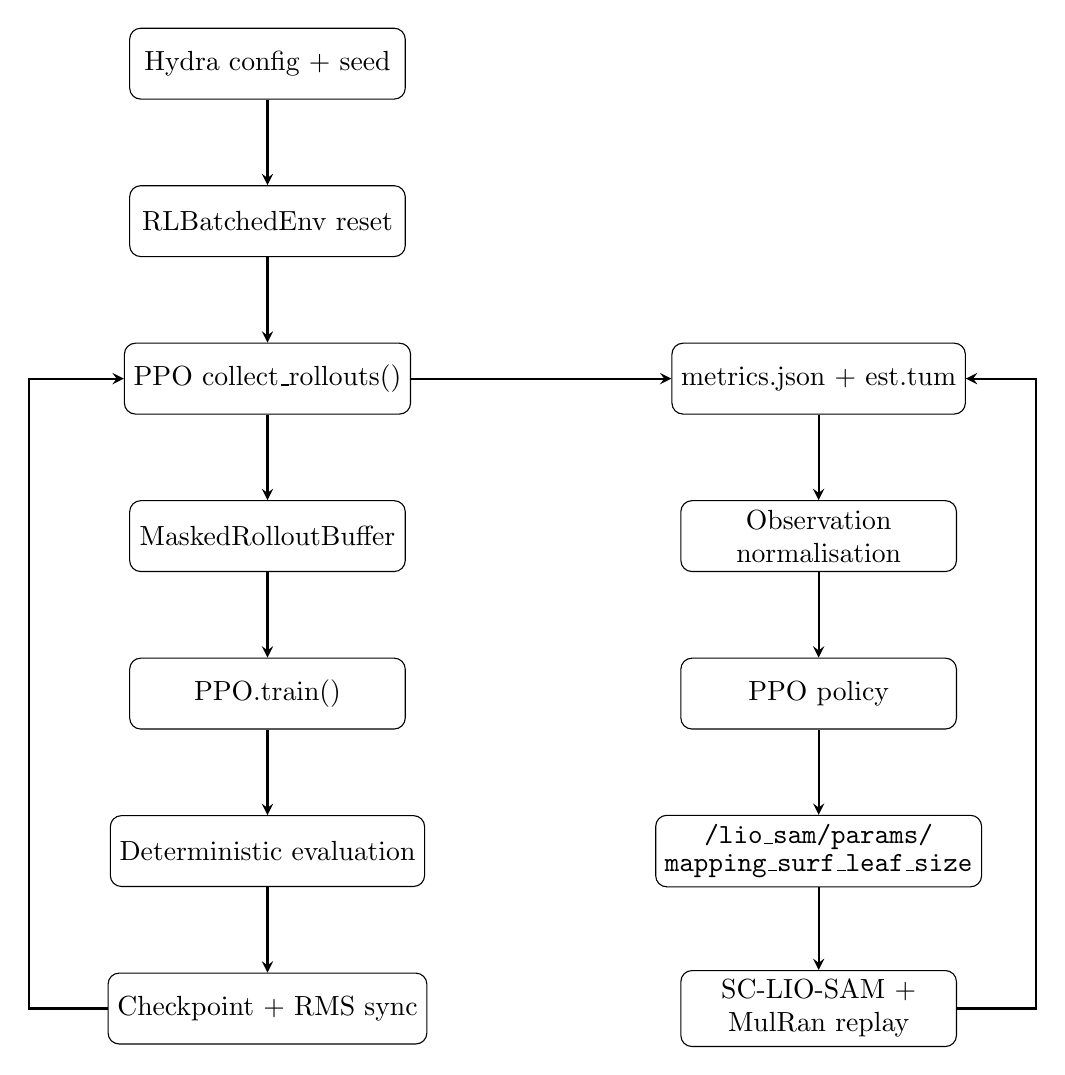
\begin{tikzpicture}[
    box/.style={rectangle, draw, rounded corners, align=center, minimum width=3.5cm, minimum height=0.9cm, fill=white},
    arrow/.style={->, >=stealth, thick}
]

% Left column - main PPO loop (using absolute coordinates)
\node[box] (start) at (0,0) {Hydra config + seed};
\node[box] (buildenv) at (0,-2) {RLBatchedEnv reset};
\node[box] (rollout) at (0,-4) {PPO collect\_rollouts()};
\node[box] (buffer) at (0,-6) {MaskedRolloutBuffer};
\node[box] (train) at (0,-8) {PPO.train()};
\node[box] (eval) at (0,-10) {Deterministic evaluation};
\node[box] (checkpoint) at (0,-12) {Checkpoint + RMS sync};

% Right column - environment interaction
\node[box] (metrics) at (7,-4) {metrics.json + est.tum};
\node[box] (obs) at (7,-6) {Observation\\normalisation};
\node[box] (action) at (7,-8) {PPO policy};
\node[box] (publish) at (7,-10) {\texttt{/lio\_sam/params/}\\[-2pt]\texttt{mapping\_surf\_leaf\_size}};
\node[box] (ros) at (7,-12) {SC-LIO-SAM +\\MulRan replay};

% Vertical arrows - left column
\draw[arrow] (start) -- (buildenv);
\draw[arrow] (buildenv) -- (rollout);
\draw[arrow] (rollout) -- (buffer);
\draw[arrow] (buffer) -- (train);
\draw[arrow] (train) -- (eval);
\draw[arrow] (eval) -- (checkpoint);

% Arrows to/from environment
\draw[arrow] (rollout) -- (metrics);
\draw[arrow] (metrics) -- (obs);
\draw[arrow] (obs) -- (action);
\draw[arrow] (action) -- (publish);
\draw[arrow] (publish) -- (ros);

% Feedback loop from ROS to metrics
\draw[arrow] (ros.east) -- ++(1,0) |- (metrics.east);

% Checkpoint feedback to rollout
\draw[arrow] (checkpoint.west) -- ++(-1,0) |- (rollout.west);

\end{tikzpicture}
\caption{PPO training pipeline showing the interaction between reinforcement learning components and the ROS-native SC-LIO-SAM environment.}
\label{fig:ppo_pipeline}
\end{figure}
This methodology produces a reproducible, ROS-native training environment where PPO policies can safely explore how \texttt{mapping\_surf\_leaf\_size} impacts SC-LIO-SAM while replaying real MulRan drives. The resulting design artefacts—hyperparameter sweep tooling, metrics exporters, and RL attention networks—form the foundation for the experiments reported in later chapters.
